%\chapter{Introducción}

\textit{Blas de Lezo y Olavarrieta} (u \textit{Olabarrieta})
\index{Blas de Lezo} (Pasajes, Guipúzcoa, 3 de febrero de
1689---Cartagena de Indias, Nueva Granada, 7 de septiembre de 1741)
fue un almirante español ---conocido por la singular estampa que le
dieron sus numerosas heridas de guerra considerado uno de los mejores
estrategas \index{armada!española} de la historia de la Armada
Española y famoso por dirigir, junto con el virrey Sebastián de
Eslava, la defensa de Cartagena de Indias durante el asedio británico
de 1741 (cfr. \cite{bci}).  \index{Cartagena!de Indias}

Blas de Lezo y Olavarrieta nació en el distrito de Pasajes de San
Pedro (Guipúzcoa) ---por entonces aún parte de San Sebastián--- a
principios de febrero de 1689 y fue bautizado en la iglesia de San
Pedro de la misma localidad el día seis siguiente. Hijo de Pedro de
Lezo y Agustina Olabarrieta, pertenecía a una familia con ilustres
marinos entre sus antepasados, en un pueblo dedicado, prácticamente en
exclusiva, a la mar. Era el tercer hijo del matrimonio, que tuvo ocho,
de los que no todos sobrevivieron a la infancia. Sus padres
pertenecían a la pequeña nobleza local, acomodada, y De Lezo contaba
con algunos antepasados importantes: su tatarabuelo había sido regidor
de la villa a comienzos de siglo, otro había sido obispo de Perú el
siglo anterior y su abuelo había sido capitán y dueño de un galeón. El
mayorazgo le privaba prácticamente de heredar bienes, así que optó por
emprender la carrera militar, como marino.

% \begin{figure}[!hbp]
% \centering
% \mbox{
% \subfigure[Rueda-piñón de un tanque Leclerc.]{
% \label{hph_01}
% 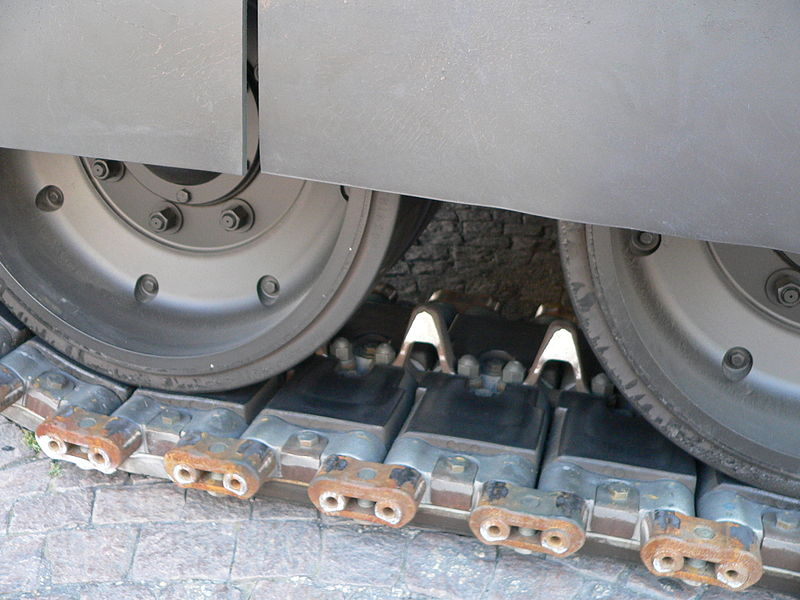
\includegraphics[width=.38\textwidth]{oruga_01.jpg}
% }
% \qquad
% \subfigure[Rueda de rodamentos de un tanque Leclerc.]{
% \label{hah}
% 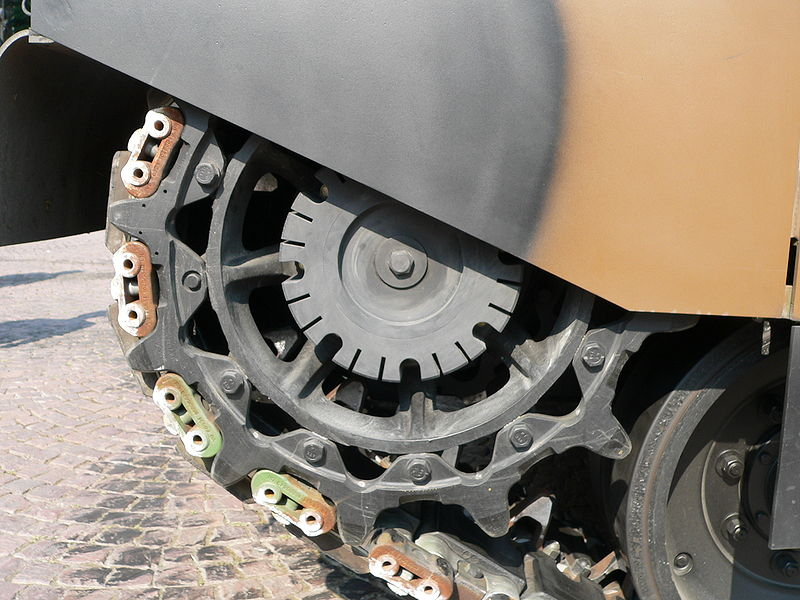
\includegraphics[width=.35\textwidth]{oruga_02.jpg}
% }
% }

% \mbox{
% \subfigure[Mi Carraro durante la carrera ]{
% \label{heh}
% 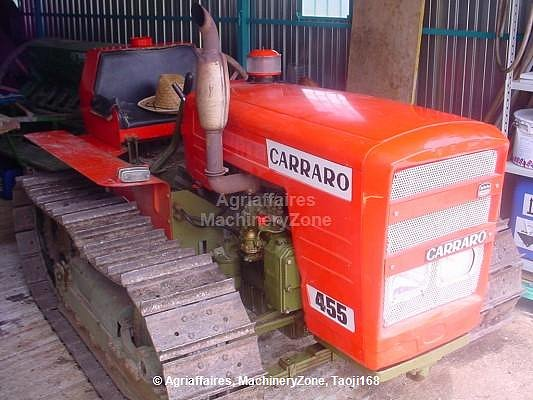
\includegraphics[width=.50\textwidth]{oruga_04.jpg}
% }
% }
% \caption{\label{fig:oruga} Detalles de un vehículo oruga.}
% \end{figure}

\begin{figure}[!hbp]
\centering
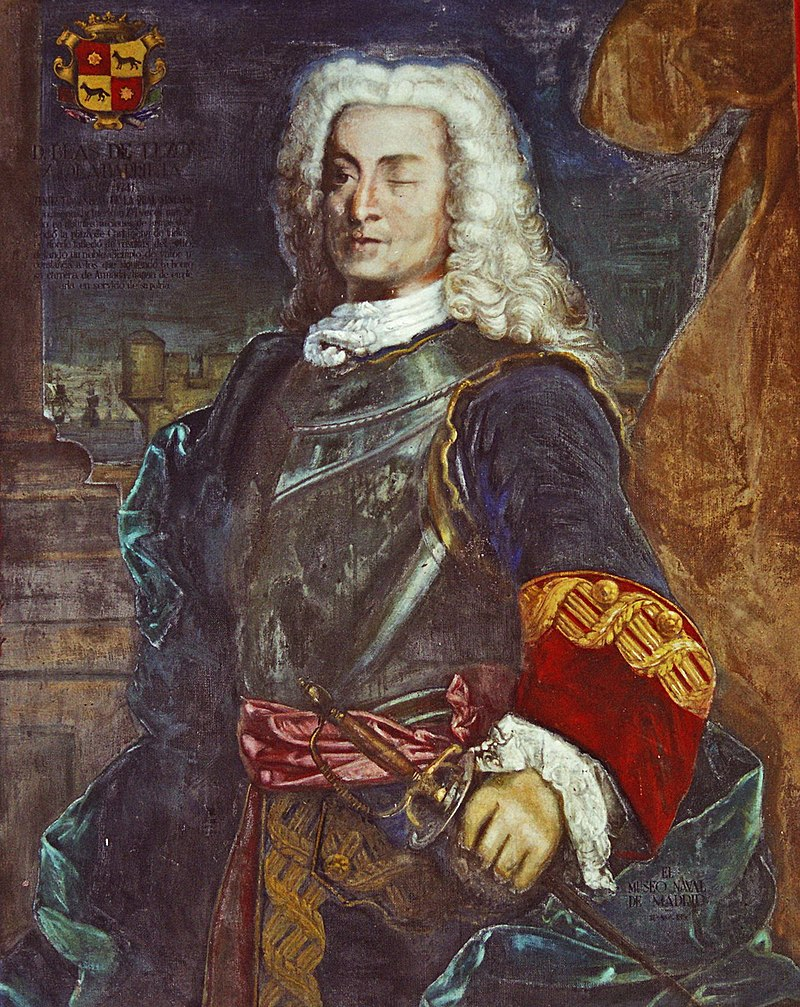
\includegraphics[width=.35\textwidth]{jpg_Don_Blas_de_Lezo_-Museo_Naval-.jpg}
\caption{\label{fig:donBlas} Don Blas de Lezo (Museo Naval de Madrid).}
\end{figure}

Se educó en el Colegio de Francia, una institución educativa para
niños de la baja nobleza de la zona donde recibió la instrucción
básica. En aquel entonces la armada francesa \index{armada!francesa}
era aliada de España en la Guerra de Sucesión, que acaba de empezar al
morir Carlos II sin descendencia. Dado que Luis XIV deseaba el mayor
intercambio posible de oficiales entre los ejércitos y escuadras de
España y Francia, Lezo se embarcó, a sus doce años, en 1702, en la
escuadra francesa ---que, en la práctica, había absorbido a la
española, en estado calamitoso, enrolándose como guardiamarina al
servicio del conde de Toulouse, Luis Alejandro de Borbón, hijo de Luis
XIV.

Se le ofreció ser asistente de cámara de la Corte de Felipe V. Rechazó
este cargo y, una vez recuperado de la pérdida de la pierna, siguió su
servicio a bordo de diferentes buques, tomando parte en las
operaciones que tuvieron lugar para socorrer las plazas de Peñíscola y
Palermo; en el ataque al navío inglés Resolution de setenta cañones
en la costa genovesa, que terminó con la quema de este; así como en
el apresamiento posterior de dos navíos enemigos en el Mediterráneo
occidental, que fueron conducidos a Pasajes y Bayona, todo ello en
1705. El mando de las presas se otorgaba como premio a los oficiales
que se habían distinguido en el servicio, como debió de hacer Lezo en
los combates de ese año.

Marino de reconocido talento y genialidad, cuya brillante carrera
aseguró el dominio marítimo del Imperio Español durante 60 años
más. Sin embargo, aunque las proezas de Blas de Lezo estén a la altura
de los más grandes héroes de la historia, es un personaje
prácticamente olvidado con el que los españoles siempre estaremos en
deuda.